\documentclass{standalone}
\usepackage{tikz}
\usetikzlibrary{arrows,shapes.gates.logic.US,shapes.gates.logic.IEC,calc}
\begin{document}
\thispagestyle{empty}
\tikzstyle{branch}=[fill,shape=circle,minimum size=3pt,inner sep=0pt]
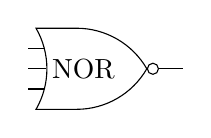
\begin{tikzpicture}   
    \node[nor gate US, draw, logic gate inputs=nnn] at (0,0) (GNOR) {NOR};
    \draw (GNOR.input 1 -| -0.7,0) -- (GNOR.input 1);
    \draw (GNOR.input 2 -| -0.7,0) -- (GNOR.input 2);
    \draw (GNOR.input 3 -| -0.7,0) -- (GNOR.input 3);
    \draw (GNOR.output) -- ++(right:3mm);
\end{tikzpicture}
\end{document}